\chapter{Security of Network Applications}

\cite{06_appsec}
\section*{Introduction}
Classic problems for modern networks:
\begin{itemize}
    \item \textcolor{Red}{Weak authentication}: usually based on passwords (password snooping, etc...) or on IP addresses (spoofing, etc...). 
    \item Data snooping / forging: data can be intercepted and modified.
    \item Shadow server / MITM.
    \item Replay, filtering. 
\end{itemize}

Security can be implemented in the transmission channel or directly in the data.

\section{Channel Security}
\begin{center}
    Security as a feature of the channel (only during the transmission).
\end{center}




\begin{multicols}{2}
    Main features:
    \begin{itemize}
        \item Peer Authentication (single or \textcolor{Blue}{mutual}), integrity and privacy only during the transit inside the communication channel.
        \item \textcolor{Red}{!!} No possibility of non-repudiation.
        \item Requires no (or small) changes to the applications.
        \item The procedures are negotiated during the connection setup (a period of insecurity).
        \item The application layer delegates the security to the lower layers (network).
    \end{itemize}
\columnbreak

\begin{figure}[H]
    \centering
    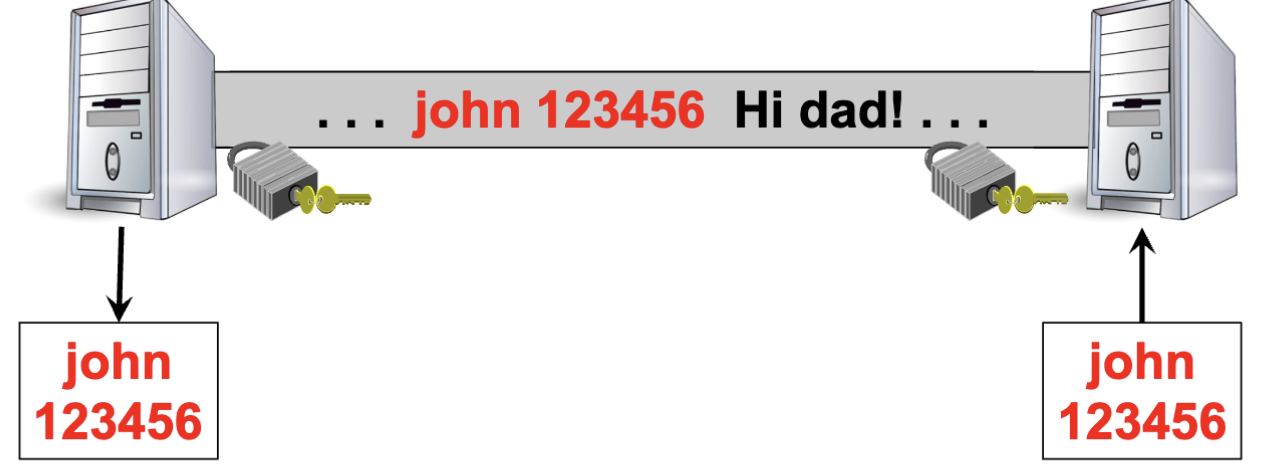
\includegraphics[width=\linewidth]{Images/Appsec/channel_security.png}
    \caption{Channel Security}
\end{figure}
\end{multicols}

\section{Data Security}
\begin{center}
    Security as a feature of the data (during the transmission and after).
\end{center}

\begin{multicols}{2}
    Main features:
    \begin{itemize}
        \item Authentication (\textcolor{Red}{!}single, only the sender), integrity and privacy self-contained in the message
        \item Possibility of non-repudiation (e.g. digital signature).
        \item Requires modifications to the applications.
        \item Much more flexibility in the security procedures.
        \item The application layer is responsible for the security.
    \end{itemize}

\columnbreak

\begin{figure}[H]
    \centering
    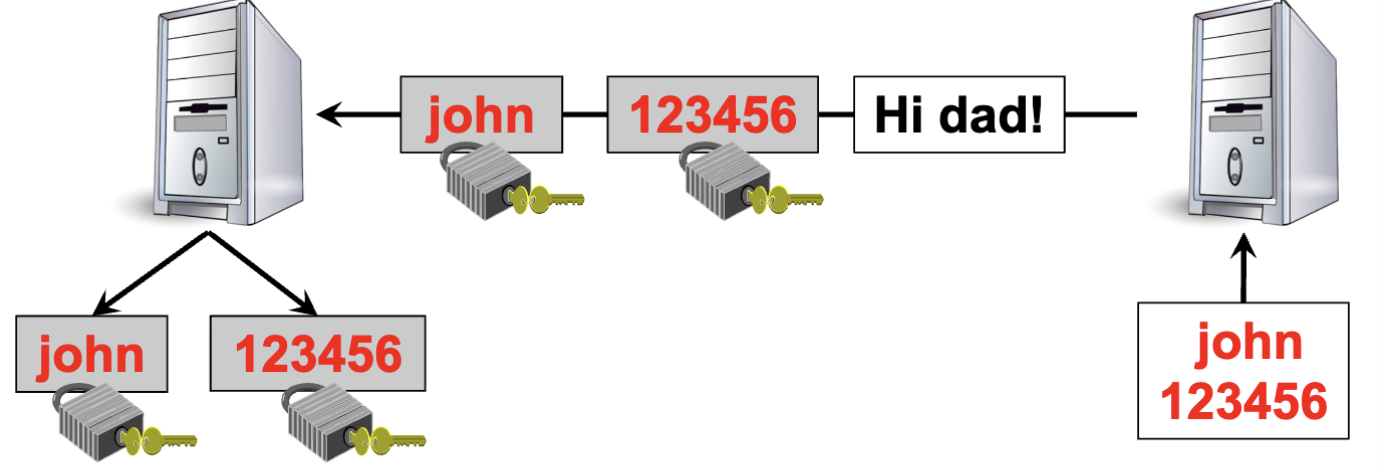
\includegraphics[width=\linewidth]{Images/Appsec/data_security.png}
    \caption{Data Security}
\end{figure}
\end{multicols}


\section{Implementing Security at the Application Layer}

\begin{multicols}{2}
    \raggedcolumns

    {\large{\textbf{Application-Internal Security}}}

    \begin{itemize}
        \item Each application implements security internally (flexibility).
        \item The common part is limited to the communication channels (socket).
        \item Possible implementation errors (inventing security protocols is not simple!).
        \item Does not guarantee interoperability.
    \end{itemize}

    \columnbreak
    \columnseprule=1pt


    {\large{\textbf{Application-External Security}}}
    
    \vspace{0.45cm}

    The session level would be the ideal one to be used to implement security functions \dots but it doesn't exist in the TCP/IP stack.

    So, a secure session (artificial) level was proposed in order to:
\begin{itemize}
\item Simplify the work of application developers.
\item Avoid implementation errors.
\item Allow the application to choose whether to use it.
\end{itemize}
    
    
\end{multicols}


\begin{multicols}{2}

    \begin{figure}[H]
        \centering
        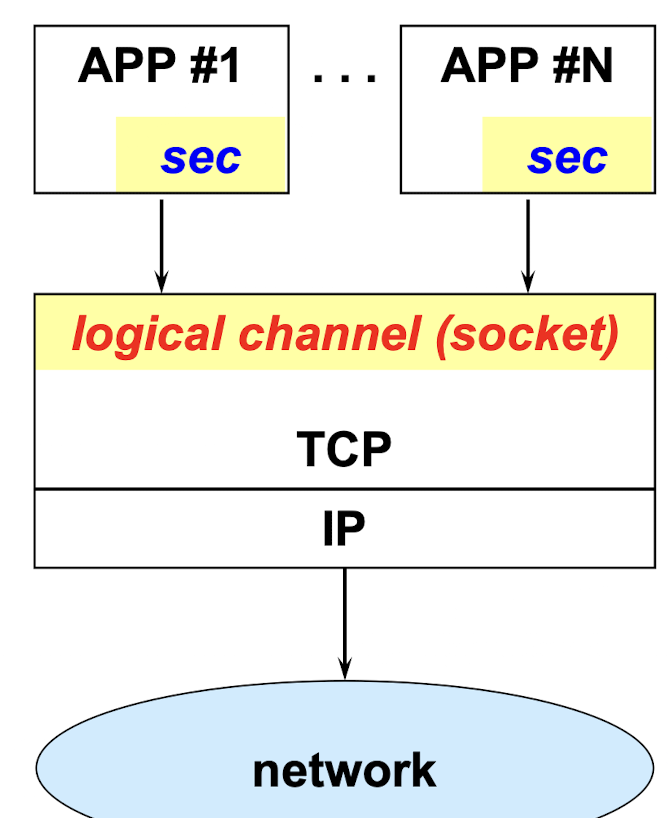
\includegraphics[width=0.5\linewidth]{Images/Appsec/sec_app.png}
        \caption{Security Internal to Applications}
    \end{figure}
    

\columnbreak

    \begin{figure}[H]
        \centering
        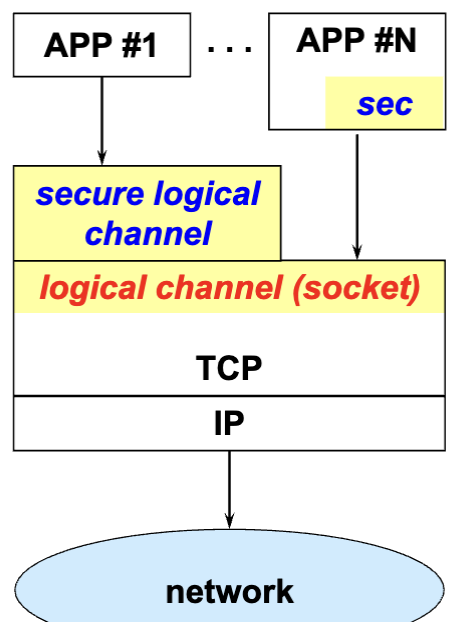
\includegraphics[width=0.44\linewidth]{Images/Appsec/external_security.png}
        \caption{Security External to Applications}
    \end{figure}


\end{multicols}

\section*{Secure Channel Protocols}
Some examples of secure channel protocols are:
\begin{itemize}
    \item SSL/TLS (Secure Sockets Layer / Transport Layer Security).
    \item SSH (Secure Shell): used for secure remote login.
    \item PCT (Private Communication Technology): proposed by Microsoft, ultimately considered a failure.
\end{itemize}

\section{TLS}
\begin{center}
    (Transport Layer Security) - was SSL (Secure Sockets Layer).
\end{center}
The high-level features of TLS are:
\begin{itemize}
    \item Secure transport channel (artificial, session level).
    \[
        \text{Each of the following properties are relevant for the exam}
    \]
    \[
        \text{Specify also the type of authentication!}
    \]
    \begin{itemize}
        \item Peer authentication (mandatory for the server and optional for the client).
        \item Message authentication and integrity (MAC-based) + Message confidentiality (encryption).
        \item Protection against replay and filtering (MID-based) attacks\footnote{Reference Appendix A}.
        \item Can implement perfect forward secrecy (PFS).
    \end{itemize}
    \item Relies on a reliable transport protocol (e.g. TCP):
    \begin{itemize}
        \item HTTP, SMTP, NNTP, FTP, TELNET and so on.
        \item The most famous secure application is HTTPS (443/TCP).
        \begin{tcolorbox}[colback=red!10!white, colframe=red!70!black, coltitle=white, title=Beware]
            HTTPS is not a protocol, it is a combination of HTTP over TLS.
            \end{tcolorbox}
    \end{itemize}
    \item Everything below TLS-1.2 is insecure and deprecated.
\end{itemize}


\subsection*{Official Ports for SSL/TLS Applications}
\begin{figure}[H]
    \centering
    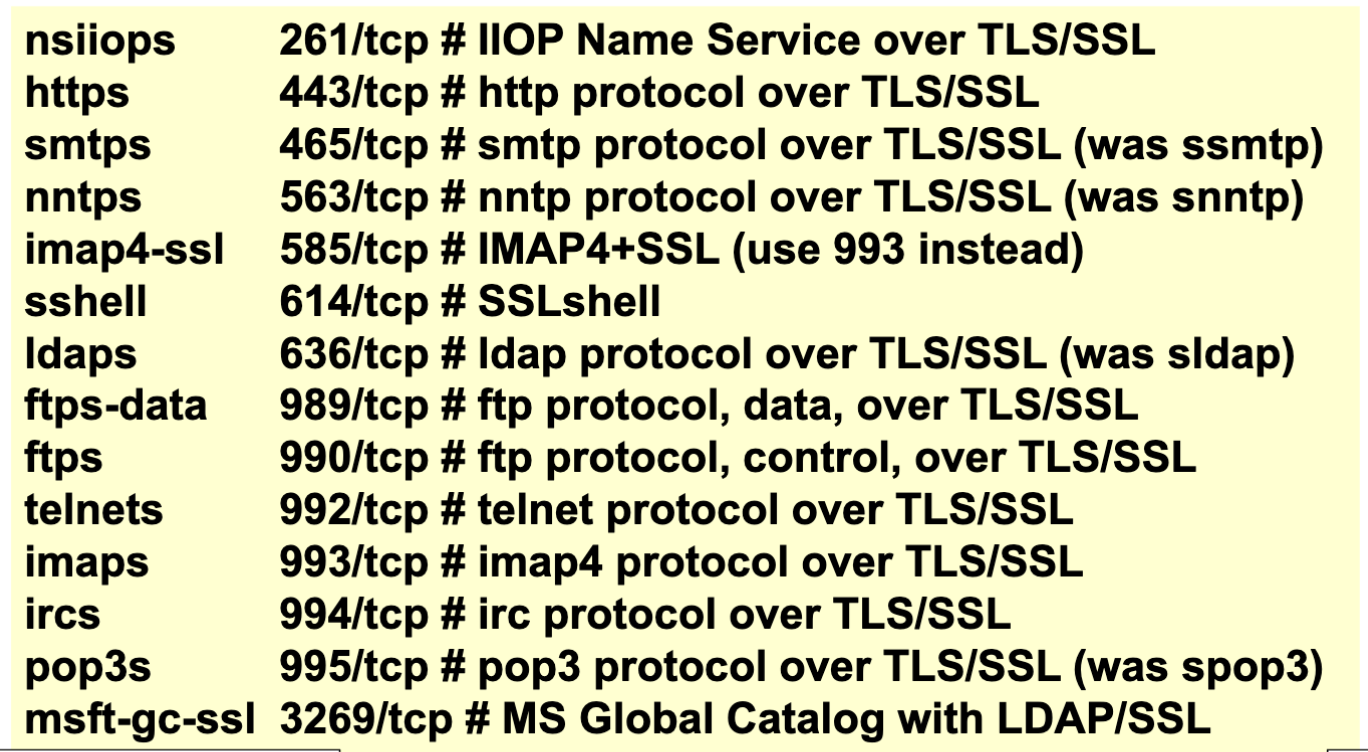
\includegraphics[width=0.5\linewidth]{Images/Appsec/ssl-tls_prot.png}
    \caption{Official Ports for SSL/TLS Applications}
\end{figure}

\begin{center}
    \textbf{Implementation Ideas}
\end{center}

\subsection{TLS - Peer Authentication}
\begin{itemize}
    \item Peer \textbf{Authentication} at channel setup: 
    \begin{itemize}
        \item The server must be authenticated (mandatory): Sends its public key certificate (X.509) \boxed{and} responds to an \uline{implicit}\footnote{The client sends the challenge encrypted with the server's public key} asymmetric challenge.
        \item The client can authenticate itself (optional): with public key, X.509 certificate and explicit challenge. This \uline{additional} authentication reduces the attack surface.
    \end{itemize}
\end{itemize}

\subsection{TLS - Data Authentication/Integrity}

For authentication and integrity of the data exchanged over the channel, TLS uses:
\begin{itemize}
    \item A keyed digest (SHA-1 or better, HMAC).
    \item An implicit MID (Message Identifier, used also in computing the keyed-digest) is used to prevent replay attacks and cancellation\footnote{Cancellation can occur when a message or transaction is invalidated. By using a unique MID, systems can avoid unintentional cancellations or false positives caused by replayed messages.}.
\end{itemize}

\subsection{TLS - Data Confidentiality}

The client generates a shared secret (pre-master secret) used for further processes in order to obtain confidentiality (e.g., using 3DES, IDEA, AES, or ChaCha20). The shared secret is exchanged with the server via public-key cryptography (RSA-based exchange) or DH (Diffie-Hellman). 

Authenticated encryption is available in TLS 1.2, while in TLS 1.3 is mandatory.

\subsection{TLS - Session ID}
\begin{center}
    Short-lived solution! (few minutes at most)
\end{center}
A typical web transaction involves the \textbf{transmission of multiple elements} between the client (e.g., a web browser) and the server. To \textbf{avoid the overhead of negotiating a new session} for each element (i.e. Many connections can be part of the same logical session), TLS uses a session ID. The session ID is a \textbf{unique identifier} that allows the client and server to \textbf{resume a previous session}.

If the client, when opening the TLS connection, sends a valid session-id, the negotiation phase is skipped, and data can be immediately exchanged over the secure channel. However, the client \textcolor{Red}{MUST} start communicating in encrypted form; otherwise, the server will reject the connection.

\begin{tcolorbox}[colback=red!10!white, colframe=red!70!black, coltitle=white, title=Beware]
    The server has the ability to reject the use of a session ID either always (for policy reasons) or after a certain time has passed since its issuance.
\end{tcolorbox}

\begin{figure}[H]
    \centering
    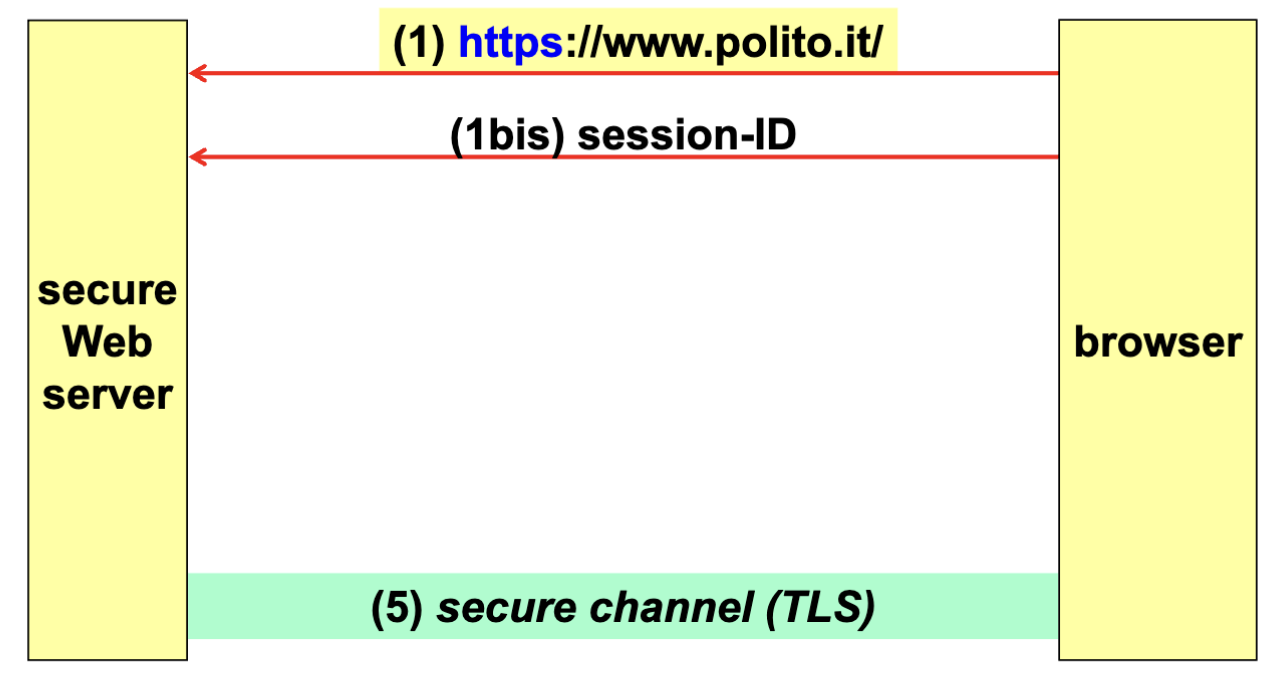
\includegraphics[width=0.6\linewidth]{Images/Appsec/handshake_tls_sess.png}
    \caption{TLS Handshake with Session ID}
\end{figure}

\subsection{TLS - Sessions and Connections}
\begin{center}
    Defintions.
\end{center}



\begin{multicols}{2}
    \raggedcolumns

    \center{\large{TLS \textbf{session}}}
    \begin{itemize}
        \item Is a logical association between client and server.
        \item Is created by the handshake protocol.
        \item Defines a set of cryptographic security parameters.
        \item Is shared by one or more TLS connections ($1:N$).
    \end{itemize}

    \columnbreak

    \center{\large{TLS \textbf{connection}}}
    \begin{itemize}
        \item Is a transient TLS channel between client and server.
        \item Is associated to one specific TLS session ($1:1$).
    \end{itemize}
    \begin{figure}[H]
        \centering
        
\includegraphics[width=\linewidth]{Images/Appsec/sess_conn.png}
        \caption{TLS Sessions and Connections}
    \end{figure}
\end{multicols}

\subsection{TLS - Architecture}
Key components of TLS architecture: 
\begin{itemize}
    \item Relies on a reliable transport protocol (e.g. TCP).
    \item Record Protocol: provides basic security services (confidentiality, integrity, etc.) and is responsible for fragmenting and reassembling messages.
    \item Change Cipher Spec Protocol: Signals a shift to the agreed encryption and hashing algorithms after the handshake.
    \[
        \text{"The handshake is over, let's start encrypting."}
    \]
    \item Alert Protocol: Used to signal errors and warnings.
\end{itemize}
    

\begin{figure}[H]
    \centering
    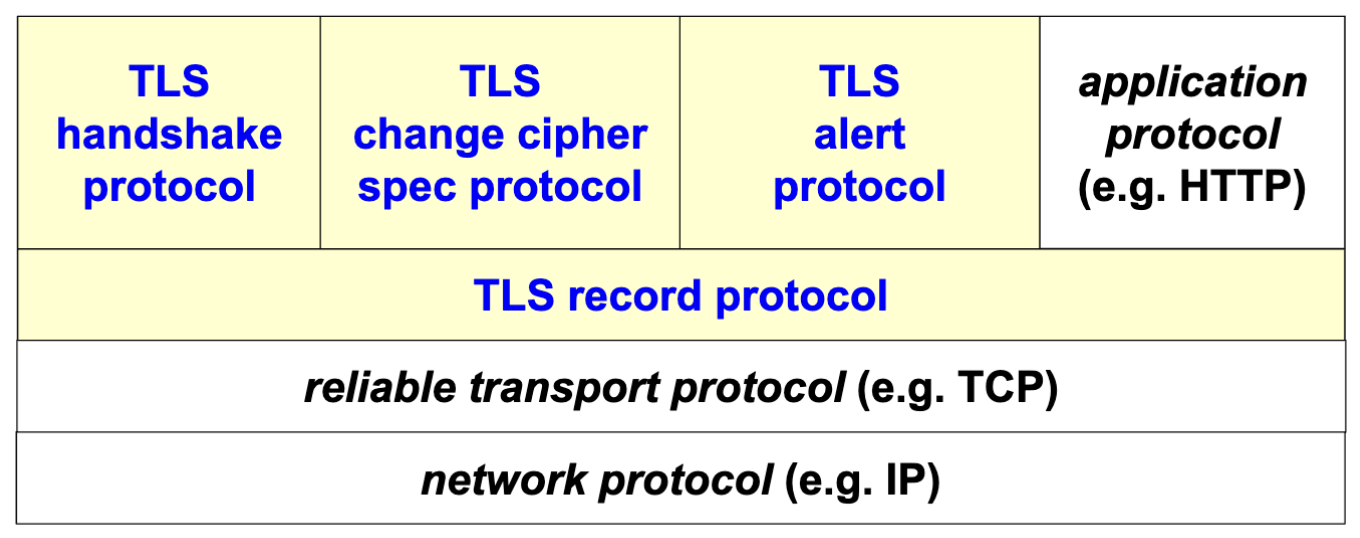
\includegraphics[width=0.5\linewidth]{Images/Appsec/tls_arch.png}
    \caption{TLS Architecture}
\end{figure}

\subsection{TLS - Record Protocol}
\begin{center}
    Authenticate-then-Encrypt (AtE) strategy.

    $enc(K_1, message, MAC(message, K_2))$
\end{center}
The steps for creating a TLS RECORD (don't consider it as a standard transport layer packet) are:

\begin{enumerate}
    \item Fragmentation: Divides the data (from the application layer or higher-level TLS protocols) into smaller blocks that can be transmitted efficiently.
    \item \textcolor{blue}{Optional} [Compression]: Reduces the size of data before encryption.
    \item Computation of MAC: The MAC is used to verify the integrity and authenticity of the data. \textcolor{Purple}{Authenticate \dots}
    \[
        MAC=\text{MAC(key, seq\_number \textcolor{Blue}{64-bit} || type || version || length || fragment)}
    \]
    There are two different keys (to prevent from replay attacks): the sender-write-key ($K_{C2S}$) and the receiver-write-key ($K_{S2C}$), both obtained from the master secret (unique for each session).

    \item Padding: Padding is added to make the total data length a multiple of the block size if necessary.
    \item Encryption: The encryption key is derived during the TLS handshake. \textcolor{Purple}{\dots then Encrypt}
    \item Record Assembly: The encrypted data is packaged into a TLS record (header+payload).
\end{enumerate}

\begin{figure}[H]
    \centering
    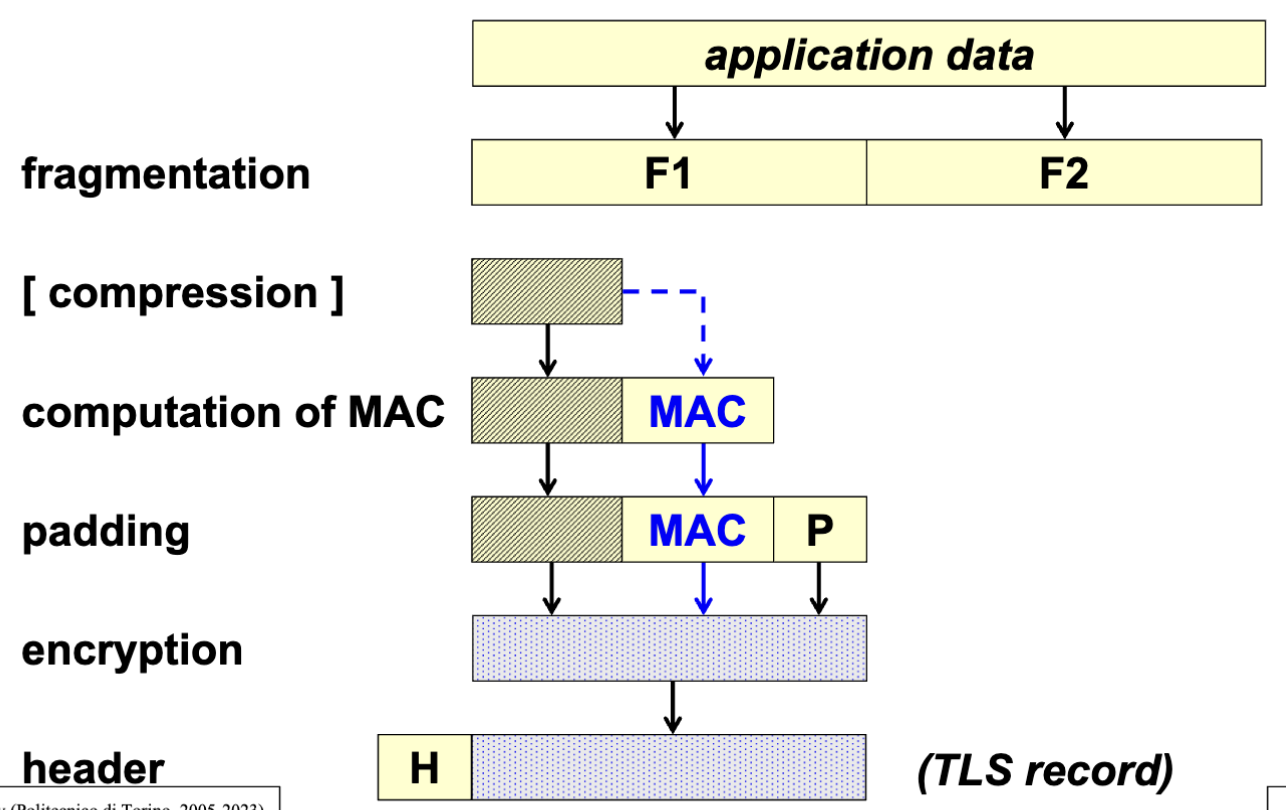
\includegraphics[width=0.5\linewidth]{Images/Appsec/record_protocol.png}
    \caption{TLS Record Protocol}
\end{figure}


\subsubsection*{Data Protection Recap}
\begin{center}
    Authenticate then Encrypt (AtE) strategy.
\end{center}
\begin{multicols}{2}
    \raggedcolumns
    Two relevant aspects:

    \vspace{0.2cm}

    \begin{enumerate}
        \item The MAC is computed before encryption. \textcolor{Purple}{Authenticate \dots}
        \item The MAC is encrypted with the data. \textcolor{Purple}{\dots then Encrypt}
    \end{enumerate}

\columnbreak

    \begin{figure}[H]
        \centering
        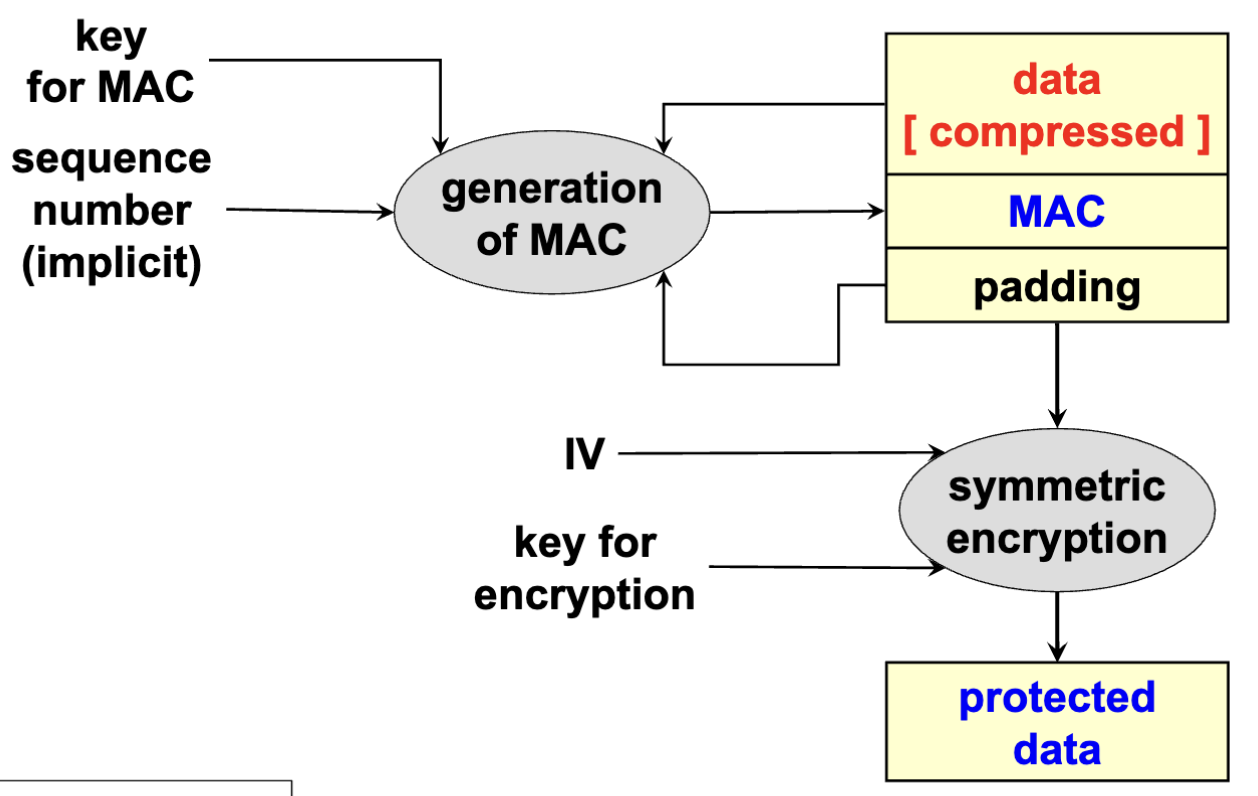
\includegraphics[width=\linewidth]{Images/Appsec/data_prot.png}
        \caption{Data Protection}
    \end{figure}
\end{multicols}

\begin{tcolorbox}[colback=red!10!white, colframe=red!70!black, coltitle=white, title=Beware]
    MAC computation and encryption are performed using the parameters exchanged during the TLS Handshake Protocol.
\end{tcolorbox}

\subsection{TLS - Handshake Protocol}
The handshake protocol is responsible for:
\begin{itemize}
    \item Establishing a secure channel between the client and server (TLS session).
    \item Negotiation of security parameters. For example a set of algorithms for confidentiality and authentication/integrity, and the TLS version to use.
    \item Exchange of random numbers between the client and server to be used for the subsequent generation of session keys.
    \item Authentication of the server (mandatory) and optionally the client.
    \item Establishment of a shared secret (pre-master secret) using public key operations or DH.
    \item Negotiation of the session ID.
\end{itemize}


\subsubsection*{Explanation of the TLS Handshake Protocol}
\begin{center}
    Simplified view of the secure channel setup, figure \ref{fig:tls_handshake}.
\end{center}
The steps:
\begin{enumerate}
    \item The browser (client) initiates a connection to the web server by requesting the website (www.polito.it) over HTTPS.
    \item Security configuration: The browser and server agree on the security settings. i.e. which encryption algorithms (ciphers) to use, protocol version (e.g., TLS 1.2 or 1.3).
    \[
        \text{"In order to speak the same language."}
    \]
    \item Certificate: The server sends its certificate to the browser to prove its identity. The certificate includes the server's public key and the domain name\footnote{The browser checks if the domain name in the certificate matches the one in the user's request. This ensures the server is legitimate.}. 
    \begin{itemize}
        \item Server Challenge / Response: This is part of the handshake to confirm (implicitly) the server's identity.
    \end{itemize} 
    \item  \textcolor{Blue}{Optional} Certificate (User): The server may require (explicitly) a client certificate to verify the user's identity.
    \begin{itemize}
        \item \textcolor{Blue}{Optional} Client Challenge / Response.
    \end{itemize} 
    \item Key exchange: The browser and server perform a key exchange to share encryption keys securely. This ensures only the browser and server can encrypt/decrypt messages.
    \item Secure Channel (TLS): At this point, the TLS handshake is complete, and a secure communication channel is established.
\end{enumerate}

\begin{figure}[H]
    \centering
    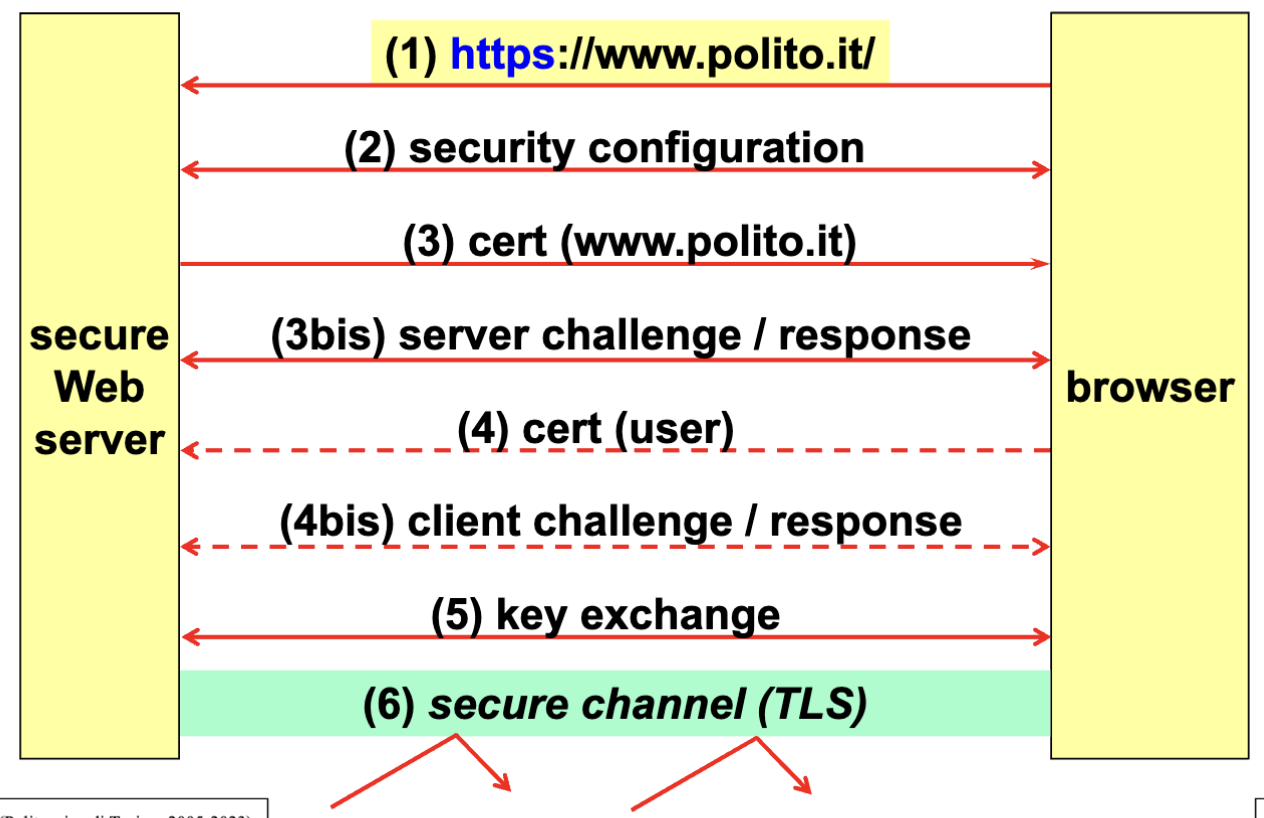
\includegraphics[width=0.6\linewidth]{Images/Appsec/tls_handshake.png}
    \caption{TLS Handshake}
    \label{fig:tls_handshake}
\end{figure}

\subsection{Keys and Sessions-Connections}
\begin{center}
    Between a server and the same client.
\end{center}

\noindent The diagram \ref{fig:rel_keys} represents how cryptographic keys are established and managed between a server and a client during secure communication.

\vspace{0.5cm}

During the TLS handshake, a \textbf{pre-master} secret is established using Public Key Cryptography (PKC) or DH. This pre-master secret, combined \uline{once} with the first connection's random numbers (generated by both the client and server during the handshake), is used to derive the \textbf{master secret}. 

\vspace{0.5cm}

Each new connection (excluding the initial handshake) uses the master secret along with \uline{newly} exchanged random values to generate unique \textbf{session keys}, which are employed to encrypt and decrypt data transmitted between the client and server and computing the MACs.

\begin{figure}[H]
    \centering
    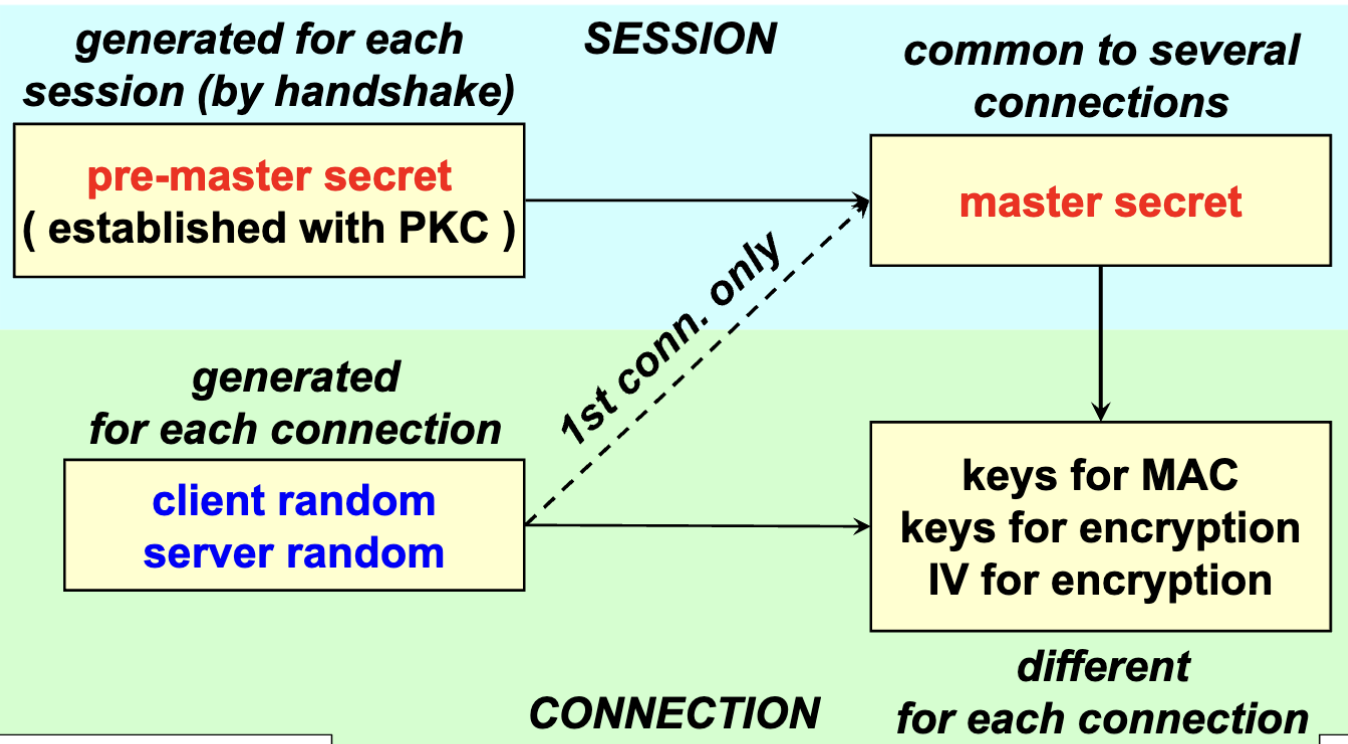
\includegraphics[width=0.6\linewidth]{Images/Appsec/rel_keys.png}
    \caption{Relationship among keys and sessions}
    \label{fig:rel_keys}
\end{figure}

\subsection{TLS - Perfect Forward Secrecy}
\begin{center}
    Introduction to PFS using TLS.
\end{center}
If a server has a certificate valid for both signature and encryption then it can be used both for authentication (via a signature) and for key exchange (via asymmetric encryption of the session key). But if:
\begin{itemize}
    \item An attacker copies all the encrypted traffic.
    \item Later discovers the (long term) private key of the server (e.g. through factorization).
\end{itemize}
\dots then the attacker can decrypt all the traffic: past, present and future.
\begin{center}
    Definition of PFS:

    \vspace{0.2cm}

    \textbf{The compromise of a private key compromises only the current \\ (and eventually future) traffic, but not the past one.}
\end{center}

\vspace{0.3cm}

This mechanism is achieved through the use of \textbf{ephemeral keys} (temporary keys) that are generated for each session and are not stored.

\begin{center}
    {\large{\textbf{"Ephemeral" Mechanisms}}}
   
    (Ephemeral keys don't provide authenticity.)
\end{center}

\noindent A \textbf{one-time key} (ephemeral key) generated on the fly and used only for a single session. The key is not stored, so even if the long-term private key is compromised, the attacker cannot decrypt past sessions.

\dots so, we obtain perfect forward secrecy.

\vspace{0.2cm}

To obtain also \textbf{authenticity}, the one-time key must be signed, using the long-term private key of the server. However, it cannot have an associated PK certificate, as the CA (Certificate Authority) process is slow and often not available online.

\vspace{0.2cm}

DH is suitable for ephemeral key exchange, RSA is slow. To mitigate RSA's slower performance, keys can be reused a few times, though this reduces the level of security compared to generating a new key for each connection.

\begin{itemize}
    \item If the (temporary or short-lived) private key is compromised, the attacker can decrypt only the traffic of the current session.
    \item Compromising the long-term private key does not compromise past sessions. Therefore, it is an issue only for authentication, but not for confidentiality.
\end{itemize}

Usually is used ECDHE (Elliptic Curve Diffie-Hellman Ephemeral).

\section{TLS 1.3}
\begin{center}
    RFC-8446 (August 2018)
\end{center}

Some of the improvements:
\begin{itemize}
    \item Only ECDHE for key exchange.
    \item Only AEAD with modern ciphers (AES, ChaCha20).
    \item Handshake redesigned for fasted and more secure setup.
\end{itemize}

\clearpage

\section{TLS Downgrade Problem}
\begin{center}
    Exposing the problem.
\end{center}
The client sends (in ClientHello) the highest supported version of TLS. The server should respond with the highest version supported by both. But an attacker can intercept the message and modify it to force the server to use an older version of TLS (weaker).

\begin{multicols}{2}
    \raggedcolumns

    \begin{center}
        Normal behavior, agreement on TLS-1.2.
    \end{center}

    \begin{verbatim}
        C>S: 3,3
        S>C: 3,3
    \end{verbatim}
    \columnbreak

    \begin{center}
        Fallback to TLS 1.1
    \end{center}
    \begin{verbatim}
        C>S: 3,3
        S>C: 3,2
    \end{verbatim}
\end{multicols}
\begin{tcolorbox}[colback=red!10!white, colframe=red!70!black, coltitle=white, title=Beware]
Initial messages, before the setup of the secure channel, are not protected by the security protocol.
\end{tcolorbox}

\noindent It's important to differentiate between:
\begin{itemize}
    \item Insecure downgrade: Some servers do not send the correct response, rather they close the connection. Then the client has no choice but to try again with a lower protocol version.
    \item Downgrade attack: An attacker sends fake server response, to force repeated downgrade until reaching a vulnerable version (e.g. SSL-3.0) then execute a suitable attack (e.g. POODLE).
\end{itemize}
The downgrade problem is not always an attack (e.g. connection with the server closed due to a network problem).

\section{TLS Fallback - Signaling Cipher Suite Value}
\begin{center}
    TLS Fallback problem solved with SCSV (RFC-7507)
\end{center}

\noindent In order to prevent the downgrade problem:
\begin{itemize}
    \item New (dummy) ciphersuite TLS\_FALLBACK\_SCSV: The client \textbf{SHOULD} send \newline \textit{TLS\_FALLBACK\_SCSV} (TLS Fallback Signaling Cipher Suite Value) when attempting to open a downgraded connection, placing it as the last cipher suite in the list.
    \item New fatal Alert value \textit{inappropriate\_fallback}: The server \textbf{MUST} respond with a fatal alert "inappropriate\_fallback" if it receives a ClientHello with the TLS\_FALLBACK\_SCSV and a version lower than the highest one supported by the server. Then the channel is close and the client should retry with its highest protocol version.
\end{itemize}

\noindent Many servers do not yet support SCSV, but most servers have fixed their bad behavior when the client requests a version higher than the supported one \dots so browsers can now disable insecure downgrade (Firefox from 2015 and Chrome from 2016).

\section{Virtual Servers and TLS}
\begin{center}
    Sam IP address used for different domains.
\end{center}
\textcolor{red}{Problem: }TLS can be challenged in virtual environments, where multiple logical server names (domains) share the same IP address. e.g.: \textit{home.myweb.it=1.2.3.4} and \textit{food.myweb.it=1.2.3.4}.

Wasn't a problem since HTTP/1.1, which allows the client to specify the domain name in the request. But it is a problem for HTTPS, where the domain name is encrypted (because TLS, transport layer security protocol, is activated before HTTP).

\vspace{0.2cm}

\noindent \textcolor{Blue}{Solution: } In order to avoid the problem, the server can use:
\begin{itemize}
    \item Collective (wildcard) certificates: the private key is shared by all servers. e.g. \textit{*.myweb.it}.
    Different browsers may react differently to this solution.

    \item Certificate with a list of servers in the SAN (subjectAltName) field: The private key is shared among all servers, and the PK certificate needs to be reissued whenever a server is added or removed.
    \begin{verbatim}
        subjectAltName:
            DNS:home.myweb.it
            DNS:food.myweb.it
            DNS:shop.myweb.it
    \end{verbatim}
    \item The SNI (Server Name Indication) \underline{extension}: The client sends the domain name in the initial message. The server can then choose the correct certificate.
    Limited support by browsers and servers.
    
\end{itemize}


\section{Application-Layer Protocol Negotiation}
\begin{center}
    ALPN (RFC-7301)
\end{center}

Application protocol negotiation (for TLS-then-proto) speeds up connection creation by avoiding additional round-trips\footnote{Such as when the channel reopens due to security configuration misunderstandings} for application negotiation.
The protocol:
\begin{itemize}
    \item C > S: ClientHello, ALPN=true + list of supported application protocols.
    \item S > C: ServerHello, ALPN=true + selected application protocol.
\end{itemize}
\begin{tcolorbox}[colback=blue!10!white, colframe=blue!50!white]
Chrome and Firefox support HTTP/2 only over TLS, and they use ALPN to negotiate the protocol.
\end{tcolorbox}

ALPN is useful also for those servers that use different certificates for the different application protocols.
\section{Datagram Transport Layer Security}
\begin{center}
    DTLS (RFC-6347)
\end{center}
DTLS applies the TLS concepts to datagram security (e.g. UDP). Does not offer the same properties as TLS. DTLS competes with other security protocols, such as IPsec and Application Security Protocols, like SIP.

\vspace{1cm}

\section*{Security SIP}
\begin{center}
    Session Initiation Protocol
\end{center}

SIP can be secured using different methods depending, also, on the transport protocol:
\begin{itemize}
    \item IPsec.
    \item TLS (only for SIP over TCP).
    \item DTLS (only for SIP over UDP).
    \item Secure SIP (SIPS).
\end{itemize}

\begin{tcolorbox}[colback=red!10!white, colframe=red!70!black, coltitle=white, title=Beware]
As usually happens in cybersecurity, there are plenty of solutions, but the choice of the security protocol depends on the specific requirements of the application.
\end{tcolorbox}

\section{HTTP Security}
\begin{center}
    \large{HTTP assumes a secure channel!}
\end{center}

Some access control features defined in HTTP/1.0 (both schemas are highly insecure!):
\begin{itemize}
    \item Basic Authentication (password-based): username and password are sent encoded (base64).
    \begin{tcolorbox}[colback=red!10!white, colframe=red!70!black, coltitle=white, title=Beware]
        Encoding brings no confidentiality!

        It is merely a transliteration of the data without requiring any knowledge of a key.
        \end{tcolorbox}
    \item Address-based authentication: The server performs access control based on the IP address of the client.
    \begin{tcolorbox}[colback=red!10!white, colframe=red!70!black, coltitle=white, title=Beware]
    Don't do access control based on the IP address, never!
    \end{tcolorbox}
\end{itemize}

HTTP/1.1 introduces Digest Authentication, based on a symmetric challenge, to replace Basic Authentication.


\clearpage

\noindent The modern HTTP authentication methods are (RFC-2617):
\begin{itemize}
    \item Basic Authentication.
    \item Digest Authentication.
\end{itemize}

\subsection{HTTP Basic Authentication}
\begin{center}
    Access control with $enc64 (username:password)$.
\end{center}
\begin{verbatim}
    C>S: GET /path/to/protected/page HTTP/1.0
    S>C: HTTP/1.0 401 Unauthorized - authentication failed
        WWW-Authenticate: Basic realm="POLITO - didattica"
    C>S: Basic czEyMzQ1NjpTZWdyZXRpc3NpbWE=
    S>C: HTTP/1.0 200 OK
        Server: Apache/1.3
        Content-type: text/html
        <html> ... protected page ... </html>
\end{verbatim}

The process:
\begin{enumerate}
    \item The client requests a protected page.
    \item The server responds with a 401 Unauthorized message and a WWW-Authenticate (\textcolor{Red}{mandatory!!}) header with the realm.
    \item The client sends the username and password encoded in base64. The credentials, when decoded, follow the format username:password.
    \begin{lstlisting}[style=bashStyle]
        #encode
        echo username:password | openssl enc -a 

        #decode
        echo YWRtaW46cGFzczEyMw== | openssl enc -a -d
    \end{lstlisting}
    \item Upon validating the credentials, the server grants access and responds with 200 OK, including the requested resource
\end{enumerate}

\begin{figure}[H]
    \centering
    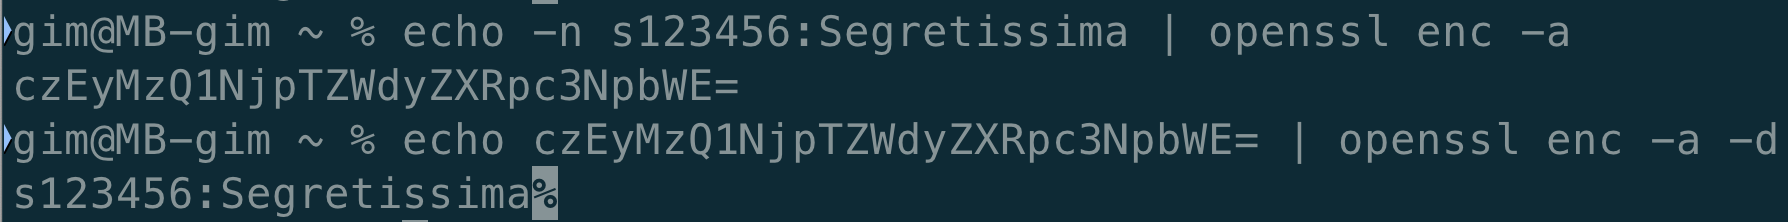
\includegraphics[width=0.6\linewidth]{Images/Appsec/basic_authN.png}
    \caption{HTTP Basic Authentication}
\end{figure}

\clearpage

\subsection{HTTP Digest Authentication}
\begin{center}
    Access control with $md5(md5(user:realm:pwd):nonce:md5(method:URI))$.
\end{center}
\begin{center}
    Access control with symmetric challenge - RFC-2069 - Technically obsoleted.
\end{center}
A more secure method than Basic Authentication, but still not secure enough for modern applications. A part of the process require the computation of a keyed digest (MD5) of the message.
\[
    HA1 = \text{md5 (A1) = md5(user":"realm":"pwd)}
\]
\[
    HA2 = \text{md5 (A2) = md5(method":"URI)}
\]

\vspace{0.3cm}

\[
    response = \text{md5 (HA1":"nonce":"HA2)}
\]

Main features:
\begin{itemize}
    \item The server uses a nonce to prevent replay attacks.
    \item The authentication server may insert a field "opaque" in the challenge, to transport state-related information (e.g. SAML token\footnote{SAML (Security Assertion Markup Language) token. Is a piece of data used for secure communication of user authentication information.}) toward the content server\footnote{System or application responsible for delivering content, such as web pages.}.
\end{itemize}

\begin{verbatim}
    C>S: GET /private/index.html HTTP/1.1
    S>C: HTTP/1.0 401 Unauthorized - authentication failed
        WWW-Authenticate: Digest realm="POLITO",
        nonce = "dcd98b7102dd2f0e8b11d0f600bfb0c093",
        opaque = "5ccc069c403ebaf9f0171e9517f40e41"
    C>S: Authorization: Digest username="lioy",
        realm="POLITO", 
        nonce="dcd98b7102dd2f0e8b11d0f600bfb0c093",
        uri="/private/index.html", 
        response="4c9d010fac372e048297160bff991883",
        opaque="5ccc069c403ebaf9f0171e9517f40e41"
    S>C: HTTP/1.0 200 OK
        Server: NCSA/1.3
        Content-type: text/html
        <html> ... protected page ... </html>
\end{verbatim}
\begin{tcolorbox}[colback=blue!10!white, colframe=blue!50!white, title=Exercise]
If you want to verify the correctness of the response, you can use:
\begin{lstlisting}[style=bashStyle]
# compute the hash of a text
echo -n <text> | openssl dgst -md5
\end{lstlisting}
    \begin{itemize}
        \item user = "lioy"
        \item realm = "POLITO"
        \item pwd = "antonio"
        \item method = "GET"
        \item uri = "/private/index.html"
        \item nonce = "dcd98b7102dd2f0e8b11d0f600bfb0c093"
        \begin{lstlisting}[style=bashStyle]
# solution
echo -n lioy:POLITO:antonio | openssl dgst -md5
#HA1 = 89e81691bc5208d6237d1b850bca4f90

echo -n GET:/private/index.html | openssl dgst -md5
#HA2 = d224a300ce6574688523c331faec896e

echo -n 89e81691bc5208d6237d1b850bca4f90:dcd98b7102dd2f0e8b11d0f600bfb0c093:d224a300ce6574688523c331faec896e | openssl dgst -md5
#response = 4c9d010fac372e048297160bff991883

        \end{lstlisting}
    \end{itemize}
\end{tcolorbox}

\subsection{HTTP and SSL/TLS}
There are two approaches:
\begin{itemize}
    \item "TLS then HTTP" (RFC-2818): The client connects to the server using TLS and then sends the HTTP request.
    \[
        \text{Content inspection is not possible!}
    \]
    \item "HTTP then TLS": The client connects to the server using HTTP and then upgrades the connection to TLS.
    \[
        \text{We see the HTTP methods until the upgrade!}
    \]
    \begin{tcolorbox}[colback=red!10!white, colframe=red!70!black, coltitle=white, title=Beware]
    "SSL then HTTP" is in widespread use, but it is not undocumented!
    \end{tcolorbox}
\end{itemize}


\noindent The two approaches are not equivalent and have an impact over applications, firewalls and IDSs. In general the most used approach is "TLS then <proto>" (e.g. HTTPS).

\section{Authentication in Web Applications}
The earlier authentication is performed, the smaller the potential attack surface. There is no need to repeat authentication across different parts of the application if the user's identity is securely propagated throughout the application.

Some web servers support a (semi-)automatic mapping between the credentials extracted from the X.509 certificate and the users of the HTTP service and/or the OS (Operative System).
\begin{tcolorbox}[colback=red!10!white, colframe=red!70!black, coltitle=white, title=Beware]
Software contains lots of vulnerabilities, and the more code you have, the more vulnerabilities (the huge the attack surface) you have. Don't ignore the HTTP basic/digest authentication and the TLS client authentication! Inside a company can be useful to apply a double authentication, or to use other modalities, such as 802.1x or IPsec (both options for "closed" groups).
\end{tcolorbox}

\begin{figure}[H]
    \centering
    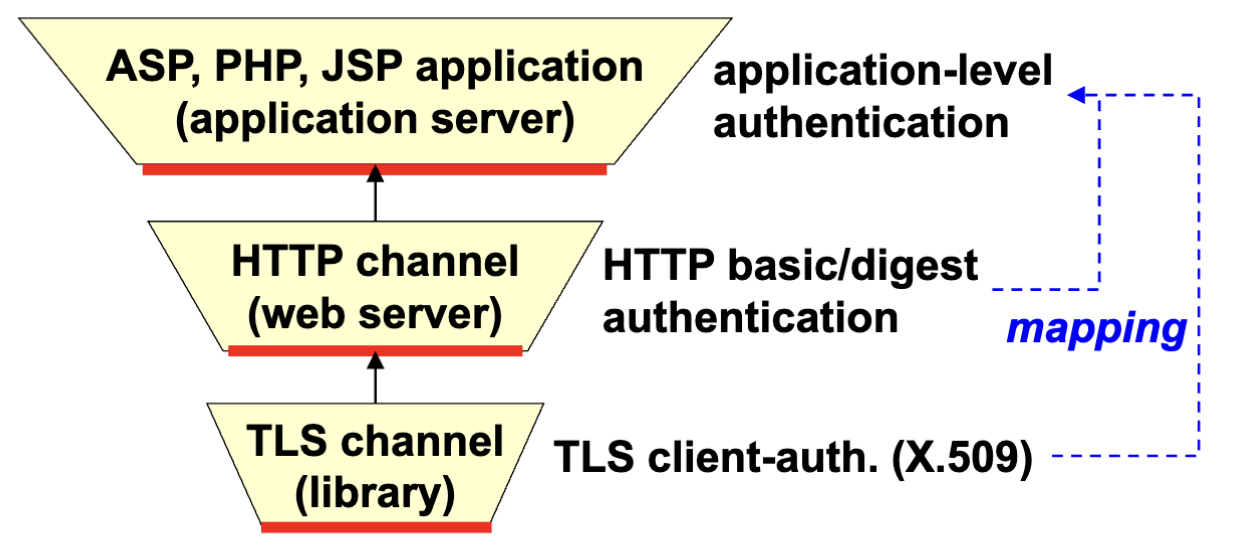
\includegraphics[width=\linewidth]{Images/Appsec/authN_app.png}
    \caption{Authentication in Web Applications}
\end{figure}

\subsection{Forms Requesting Credentials?}
Technically speaking, it's not important the security of the page containing the form (e.g. http://www.ecomm.it/login.html), but the security of the page that receives the credentials. The form page can be compromised, but the credentials are sent to the server, and the server must be secure.

\vspace{0.2cm}

Because the actual security depends on the URI of the method used to send username and password. For example in the case of a form: <form ... \textit{action="https://www.ecomm.it/login.php"}>

\vspace{0.2cm}

Psychologically, it is very important that the form page is secure, as few users have the technical knowledge to verify the HTTP URI (e.g., using browser inspection tools) or the method used to send credentials.

\subsection{HTTP Strict Transport Security}
\begin{center}
    HSTS (RFC-6797) - HTTPS only sites.
\end{center}

HTTP server declares that its interaction with UA (User Agent) must be done only through HTTPS (Prevents protocol downgrade and cookie hijacking).

\vspace{0.2cm}

\noindent Key features:
\begin{itemize}
    \item Valid only in HTTPS responses.
    \item Expiration renewed at every access.
    \item May include subdomains (recommended).
    \item May be preloaded in the browser: dangerous and difficult to remove. 
    
    The \href{https://hstspreload.org/}{preload list} is maintained by Google and used by many browsers.
\end{itemize}

\begin{center}
    \textbf{HSTS Syntax and Examples}
\end{center}

The syntax is:
\begin{verbatim}
    Strict-Transport-Security:
        max-age=<expire-time-in-seconds>
        [; includeSubDomains]
        [; preload]
\end{verbatim}

\begin{lstlisting}[style=bashStyle]
#first example
curl -s -D- https://www.paypal.com/ | fgrep -i strict
#output: Strict-Transport-Security: 
#               max-age=63072000 
#               ; includeSubDomains
#               ; preload

#second example
curl -s -D- https://accounts.google.com/ | grep -i strict
#output: Strict-Transport-Security:
#               max-age=31536000
#               ; includeSubDomains
\end{lstlisting}

\clearpage

\section{HTTP Public Key Pinning (HPKP)}
\begin{center}
    RFC-7469 - deprecated.

    Used to prevent MITM attacks.
\end{center}
An HTTPS site specifies the digest of its own public key and/or one or more Certificate Authorities (CAs) in its chain (excluding the root). The User Agent (UA) caches this digest and will refuse to connect to a site presenting a different digest.

\begin{itemize}
\item This is a TOFU (Trust On First Use) mechanism.
\item It becomes dangerous if the digest is lost or compromised.
\item There are challenges with key updates; always include at least one backup digest.
\item There's a URI to report violations.
\item Enforcing or report-only mode (UA does not block the violation but still sends a report).
\end{itemize}

…so the server sends its certificate and public key to allow the client to verify whether the server is legitimate or not (as attackers may obtain fraudulent certificates).

\begin{center}
    \textbf{HPKP Syntax and Examples}
\end{center}

The syntax is:
\begin{verbatim}
    Public-Key-Pins:
        pin-sha256="<base64-sha256-of-public-key>";
        max-age=<expire-time-in-seconds>
        [; includeSubDomains]
        [; report-uri="<reporting-URI>"]

    Public-Key-Pins-Report-Only:
        pin-sha256="<base64-sha256-of-public-key>";
        max-age=<expire-time-in-seconds>
        [; includeSubDomains]
        [; report-uri="<reporting-URI>"]
\end{verbatim}

\begin{lstlisting}[style=bashStyle]
#first example
curl -s -D - https://scotthelme.co.uk/ | fgrep -i public-key 
#output: public-key-pins:
#           pin-sha256="9dNiZZueNZmyaf3pTkXxDg8J3j5J9z8J9z8J9z8J9z8=";
#           .
#           .
#           includeSubDomains; max-age=5184000;
#           report-uri="https://scotthelme.report-uri.io/r/default/hpkp/enforce"
#           .
#       public-key-pins-report-only:
#           pin-sha256="9dNiZZueNZmyaf3pTkXxDg8J3j5J9z8J9z8J9z8J9z8=";
#           .
#           max-age=5184000;
#           report-uri="https://scotthelme.report-uri.io/r/default/hpkp/reportOnly"

\end{lstlisting}

\section{E-Payment Systems}
\begin{center}
    Security in e-commerce.
\end{center}

What happened in the past:
\begin{itemize}
    \item Failure of digital cash due to technical and legal reasons.
    \item Failure of a dedicated payment protocol (SET - Secure Electronic Transaction) caused by technical and organizational challenges.
    \begin{tcolorbox}[colback=red!10!white, colframe=red!70!black, coltitle=white, title=Beware]
    Providing users with specialized software can compromise the security of the system.
    \end{tcolorbox}
    \item Currently, the most widely used approach is transmitting credit card numbers over a TLS channel. However, this does not guarantee protection against fraud: in the past, VISA Europe reported that internet transactions accounted for about $50\%$ of fraud attempts, despite representing only $2\%$ of total transactions.
\end{itemize}

\subsection{Web-Based Payment Architecture}
The figure \ref{fig:wb_pay} shows the architecture of a web-based payment system. The steps are:
\begin{enumerate}
    \item The merchant presents the products or services on their website for the cardholder to browse.
    \item The cardholder places an order through the merchant's website, initiating the payment process.
    \item The merchant redirects the cardholder to a payment gateway\footnote{The payment gateway acts as a trusted intermediary between the merchant and the financial world, simplifying integration and handling sensitive payment details securely.} or a virtual POS (Point of Sale). This ensures sensitive payment details are handled securely.
    \item The cardholder enters its credit card information directly on a secure webpage provided by the payment gateway. This happens over a TLS-encrypted connection to ensure data confidentiality.
    \item The credit card data is securely transmitted from the cardholder to the payment gateway via TLS. This ensures the data cannot be intercepted during transmission.
    \item The payment gateway forwards the credit card data to the payment network (e.g., Visa, Mastercard) to verify the validity of the card and its details (e.g., available funds, card status).
    \item The payment network responds to the payment gateway with the result of the transaction (e.g., approval or denial).
    \item The payment gateway informs the merchant whether the payment was successful. If approved, the merchant proceeds with the transaction (e.g., delivering goods or services).
\end{enumerate}

\begin{figure}[H]
    \centering
    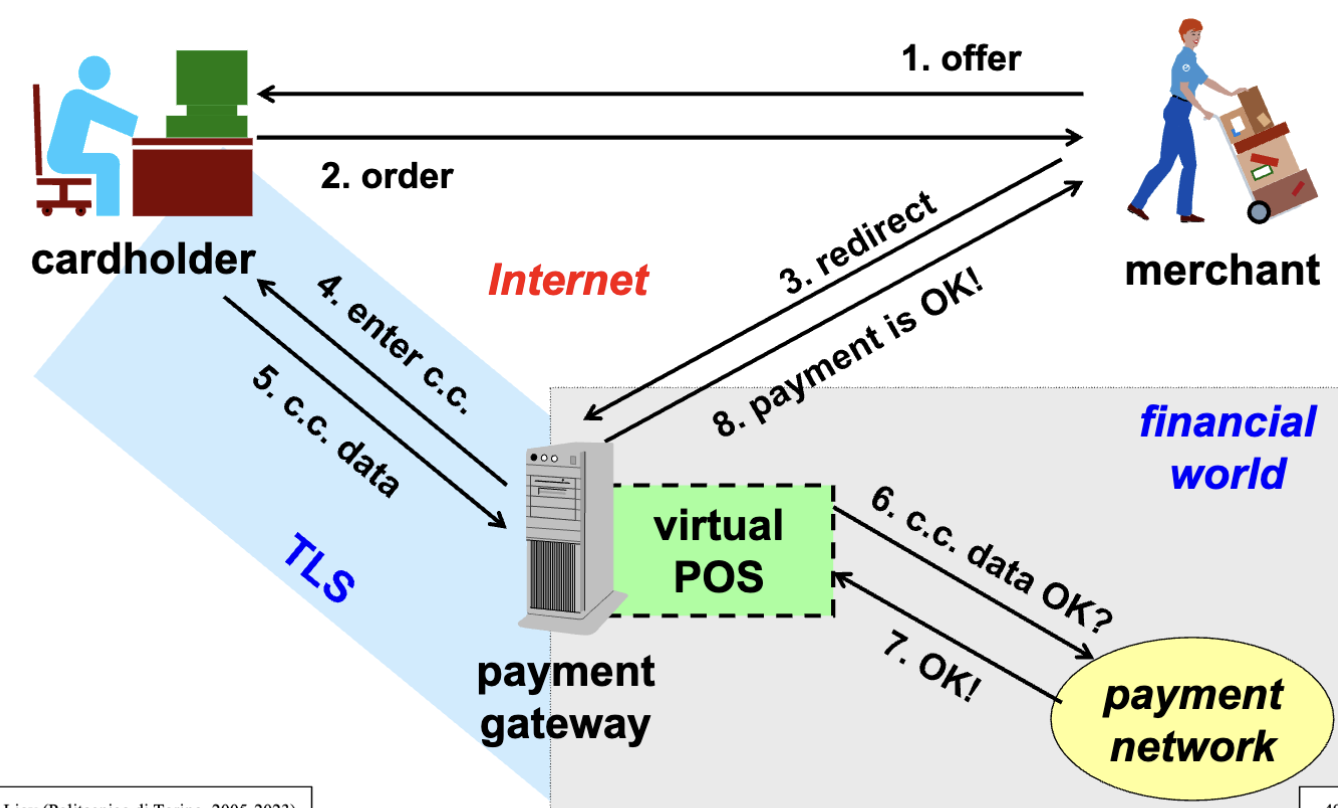
\includegraphics[width=\linewidth]{Images/Appsec/wb_pay.png}
    \caption{Web-Based Payment Architecture}
    \label{fig:wb_pay}
\end{figure}

\begin{center}
    \textbf{Assumptions}
\end{center}

\begin{itemize}
    \item The buyer owns a credit card and is willing to use it.
    \item The buyer has a TLS-enabled browser.
\end{itemize}
\begin{center}
    \textbf{Consequences (possible problems)}
\end{center}
\begin{itemize}
    \item The effective security depends upon the configuration of both the server and the client.
    \item The payment gateway has all the information (payment + goods) while merchant knows only info about the goods.
\end{itemize}

\clearpage 

\subsection{Payment Card Industry Data Security Standard}
\begin{center}
    PCI DSS
\end{center}

Main features:
\begin{itemize}
    \item Required by all credit card issuers for Internet-based transactions.
    \item Very detailed technical prescriptions compared to other security standards (e.g. HIPAA - Health Insurance Portability and Accountability Act).
\end{itemize}

\begin{center}
    \subsubsection*{PCI DSS Prescriptions - Rules}
\end{center}


    {\center{\large{\textbf{Design, build and operate a protected network}}}}
\begin{enumerate}
    \item Install and maintain a firewall configuration to protect cardholder data.
    \item Do not use pre-defined system password or other security parameters set by the manufacturer.
    {\center{\large{\textbf{Protect the cardholders' data}}}}
    \item Protect stored cardholders' data.
    \item Encrypt the cardholders' data when transmitted across an open public network.
    {\center{\large{\textbf{Establish and follow a program for vulnerability management}}}}
    \item Use and regularly update antivirus software or programs.
    \item Develop and maintain secure systems and applications.
    {\center{\large{\textbf{Implement strong access control measures}}}}
    \item Limit the access to the cardholders' data to a "need-to-know"\footnote{Only individuals or systems that require access to cardholder data to perform their specific duties should have access. } basis.
    \item Assign a single unique ID to each user.
    \item Limit physical access to the cardholders' data.
    {\center{\large{\textbf{Design, build and operate a protected network}}}}
    \item Track and monitor all access to network resources and cardholders' data.
    \item Regularly test security systems and processes.
    {\center{\large{\textbf{Design, build and operate a protected network}}}}
    \item Adopt a Security Policy: Clearly define a security policy that outlines the rules, procedures, and responsibilities for ensuring data protection and secure operations. 
\end{enumerate}

